\documentclass[11pt,a4paper]{article}
\usepackage[T1]{fontenc}
\usepackage[utf8]{inputenc}
\usepackage[polish]{babel}
\usepackage{amsmath}
\usepackage{amsfonts}
\usepackage{graphicx}
\author{Kamil Kuczaj}
\title{Sprawozdanie z Laboratorium 8 - Pomiar czasu algorytmów BFS i DFS grafu nieskierowanego.}
\date{\today}
\begin{document}

\maketitle

\section{Wstęp}
\hspace{4ex}Zadaniem na laboratorium był pomiar czasu przeszukania grafu korzystając z dwóch algorytmów:
\begin{enumerate}
\item DFS (\textit{Depth First Search}, czyli tzw. przeszukiwanie wgłąb grafu
\item BFS (\textit{Breadth First Search}, czyli tzw. przeszukiwanie wszerz grafu.
\end{enumerate} Wg teorii oba algorytmy mają złożoność obliczeniową równą O(E), gdzie E jest liczbą krawędzi w grafie (\textit{ang. Edge}. Zdecydowano się na implementację grafu na postawie listy sąsiedztwa. Jest to trudniejsza konstrukcja, jednak oba algorytmy będą szybsze na takiej strukturze. Iterowanie po liście jest znacznie szybsze niż iterowanie po tablicy oraz pozwala zaoszczędzić wiele pamięci operacyjnej.\\\\W naszym przypadku mieliśmy załadować kolejno $10^1$, $10^3$, $10^5$, $10^6$ oraz sprawdzić czas wyszukiwania znanego elementu. Sposób generacji polegał na tym, aby stworzyć n wierzchołków, połączyć każdy wierzchołek z następnym krawędzią o wadze równej 1. Łącząc ostatni wierzchołek z pierwszym powstawało koło. Następnie połowa wierzchołków pseudolosowo (bibilioteka \textit{<csdtdlib>}) generowała krawędź o wadze 1 z innym wierzchołkiem
\section{Specyfikacja komputera}

\begin{center}
	\begin{tabular}{| r | c |}
	\hline
	Wersja kompilatora \textit{g++} & 4.8.4 \\ \hline
	System & Ubuntu 14.04.4 \\ \hline
	Procesor	 & Intel Core i5 2510M 2.3 GHz \\ \hline
	Pamięć RAM & 8 GB DDR3 1600 MHz \\ \hline
	Dysk twardy & HDD (5400 obr./min) \\ \hline
	Rozmiar zmiennej \textit{int} & 4 bajty \\ \hline
	\end{tabular}
\end{center}

\section{Pomiary oraz ich interpretacja}



%\begin{figure}[htbp]
%\begin{center}
%	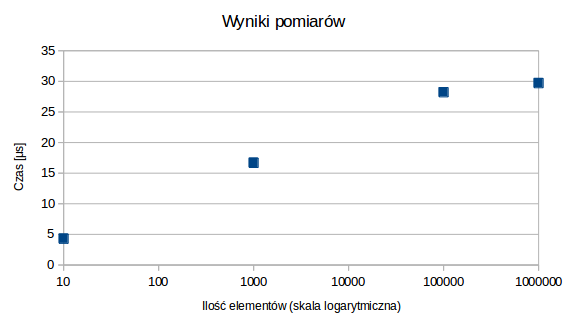
\includegraphics[scale=0.7]{wykres.png}
%\end{center}
%\end{figure}


\section{Wnioski}
\hspace{4ex} Algorytmy BFS i DFS były wadliwe, więc nie zdołano zmierzyć czasu ich realizacji.
\end{document}